%/**********************************************************************/
%		第1章:序論
%/**********************************************************************/
\pagenumbering{arabic}
\chapter{序章}
\label{lbl_chptr1}

近年の技術的進歩や流行と研究の関連性について言及する

%/**********************************************************************/
%		研究背景
%/**********************************************************************/

\section{研究背景}
\label{lbl_cp1_haikei}

研究背景を書く。

	\begin{table}[tbh]
%		\vspace{-4mm}
		\caption{IT市場の予測.}
%		\ecaption{Implementation results of FMCAM.}
%		\vspace{-3mm}
			\begin{center}
				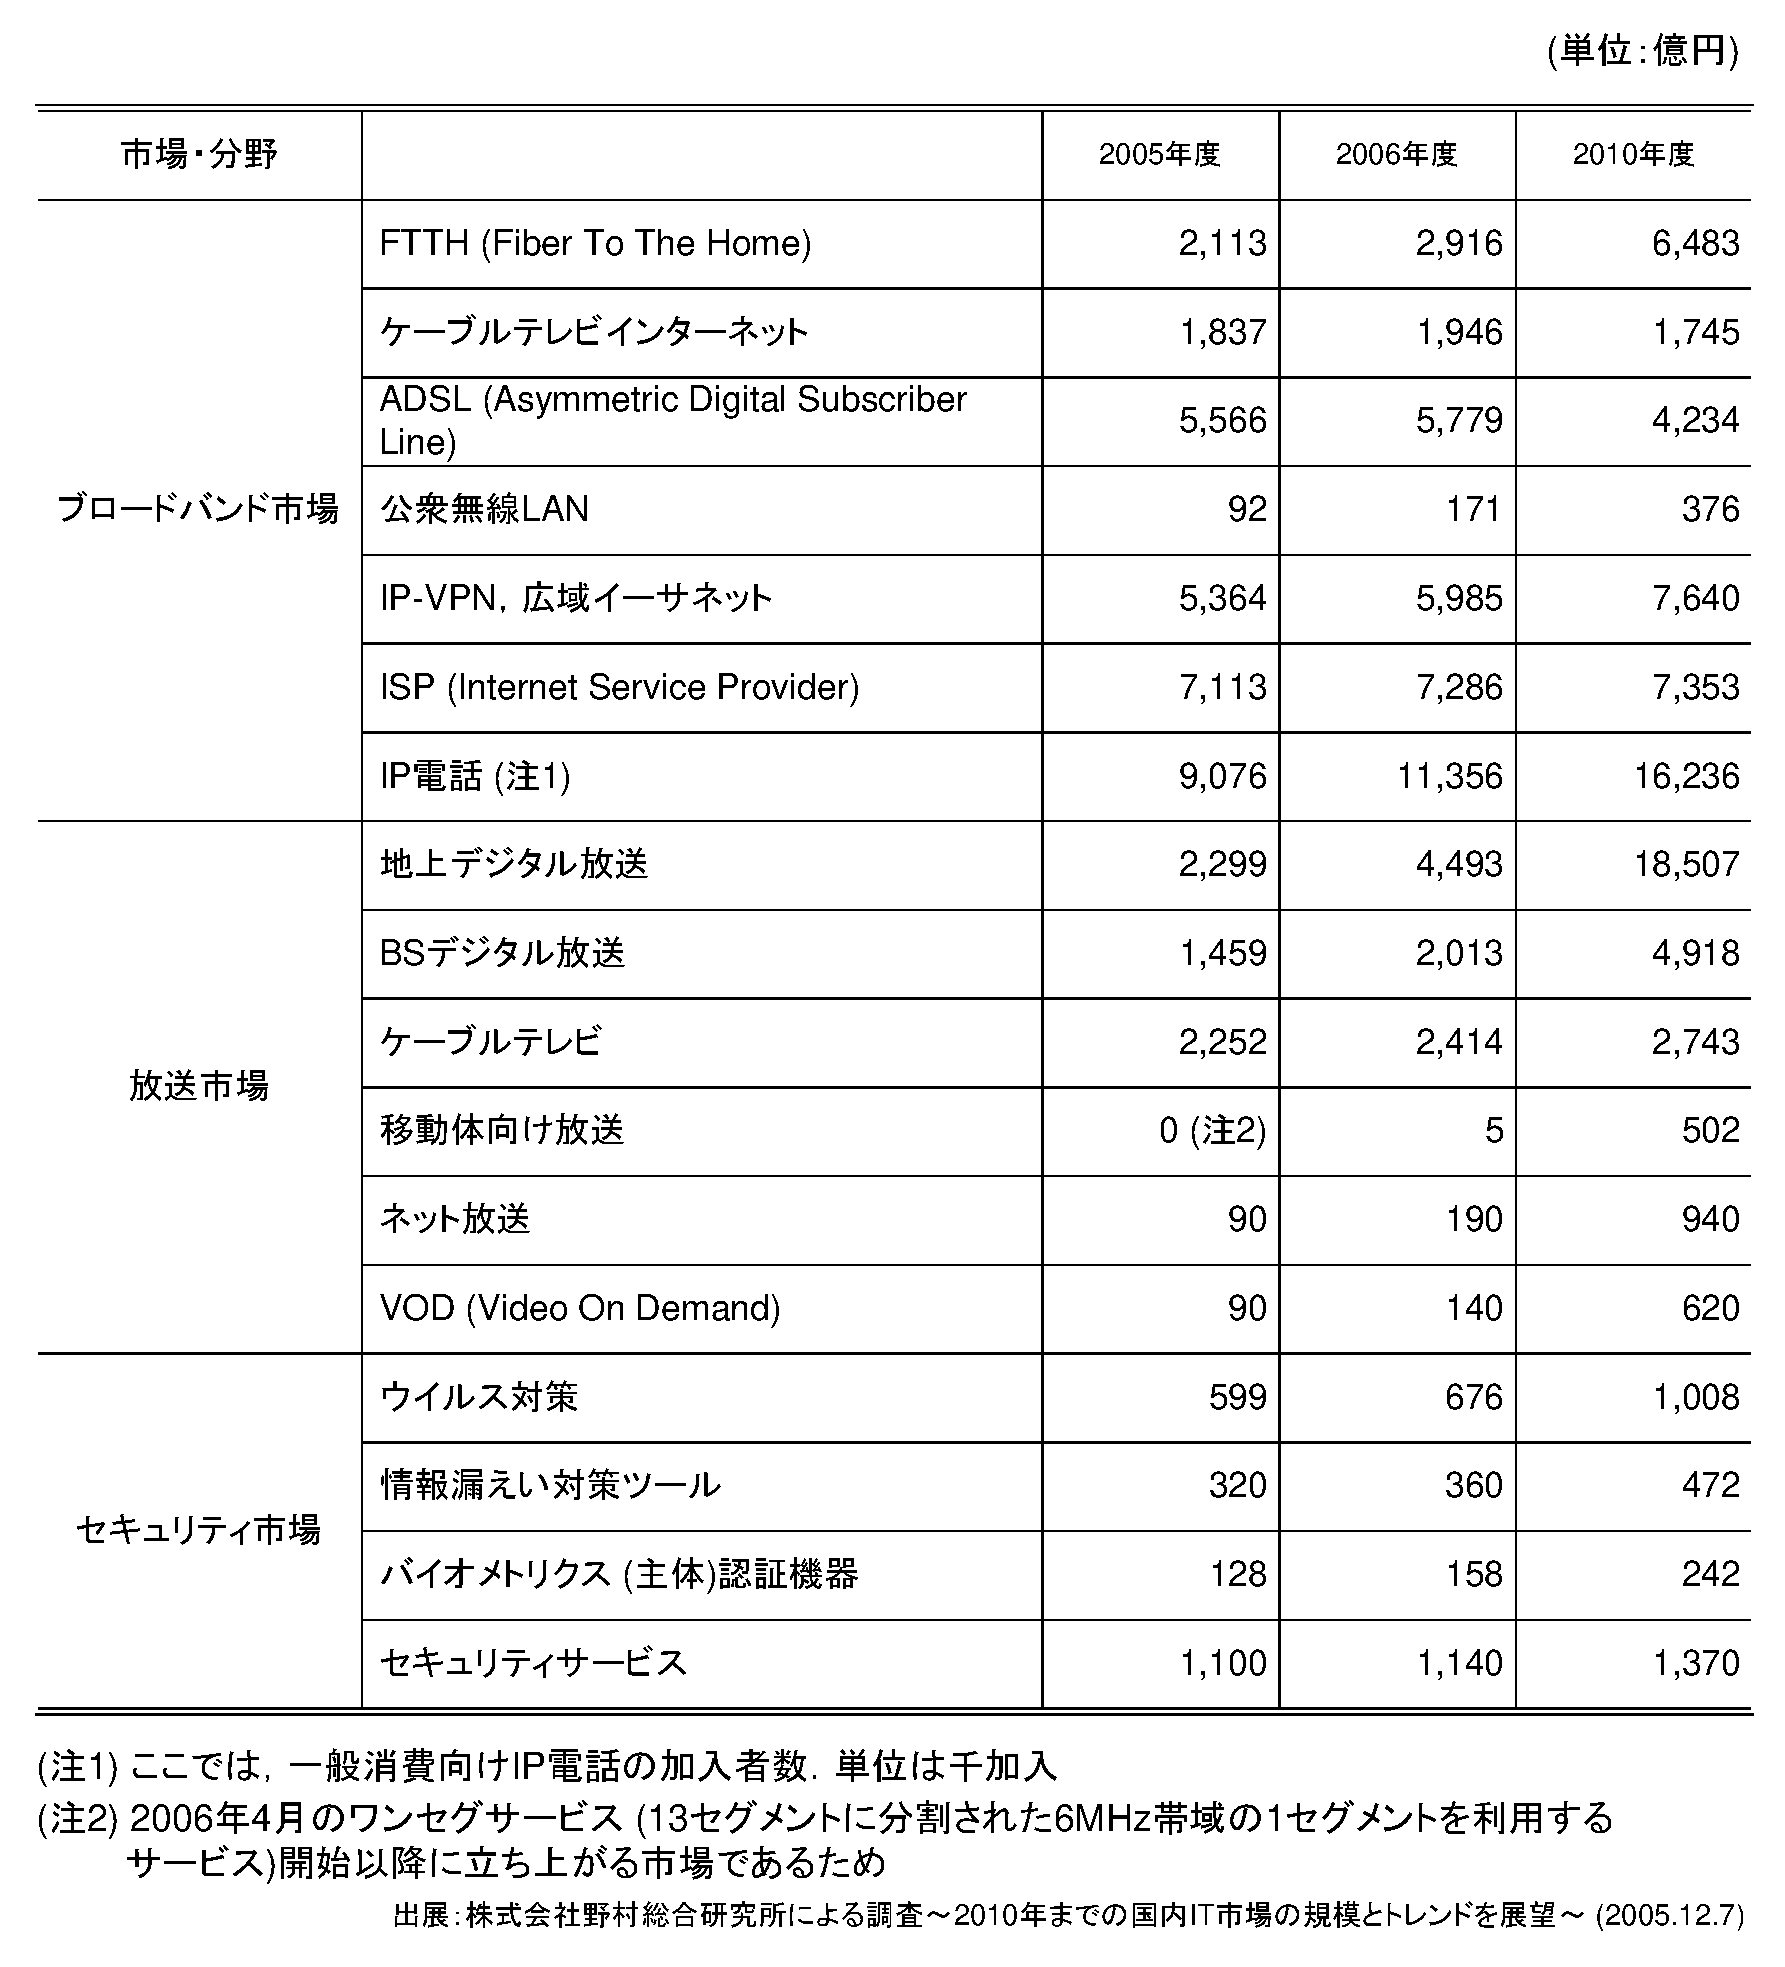
\includegraphics[width = 14cm,  height = 14cm,  keepaspectratio,  clip]{./pics/nomura.eps}
			\end{center}
		\label{nomura}
%		\vspace{-10mm}
	\end{table}%

	\begin{table}[tbh]
%		\vspace{-4mm}
		\caption{携帯電話,eビジネスライフ及びプラットフォーム各市場の予測.}
%		\ecaption{Implementation results of FMCAM.}
%		\vspace{-3mm}
			\begin{center}
				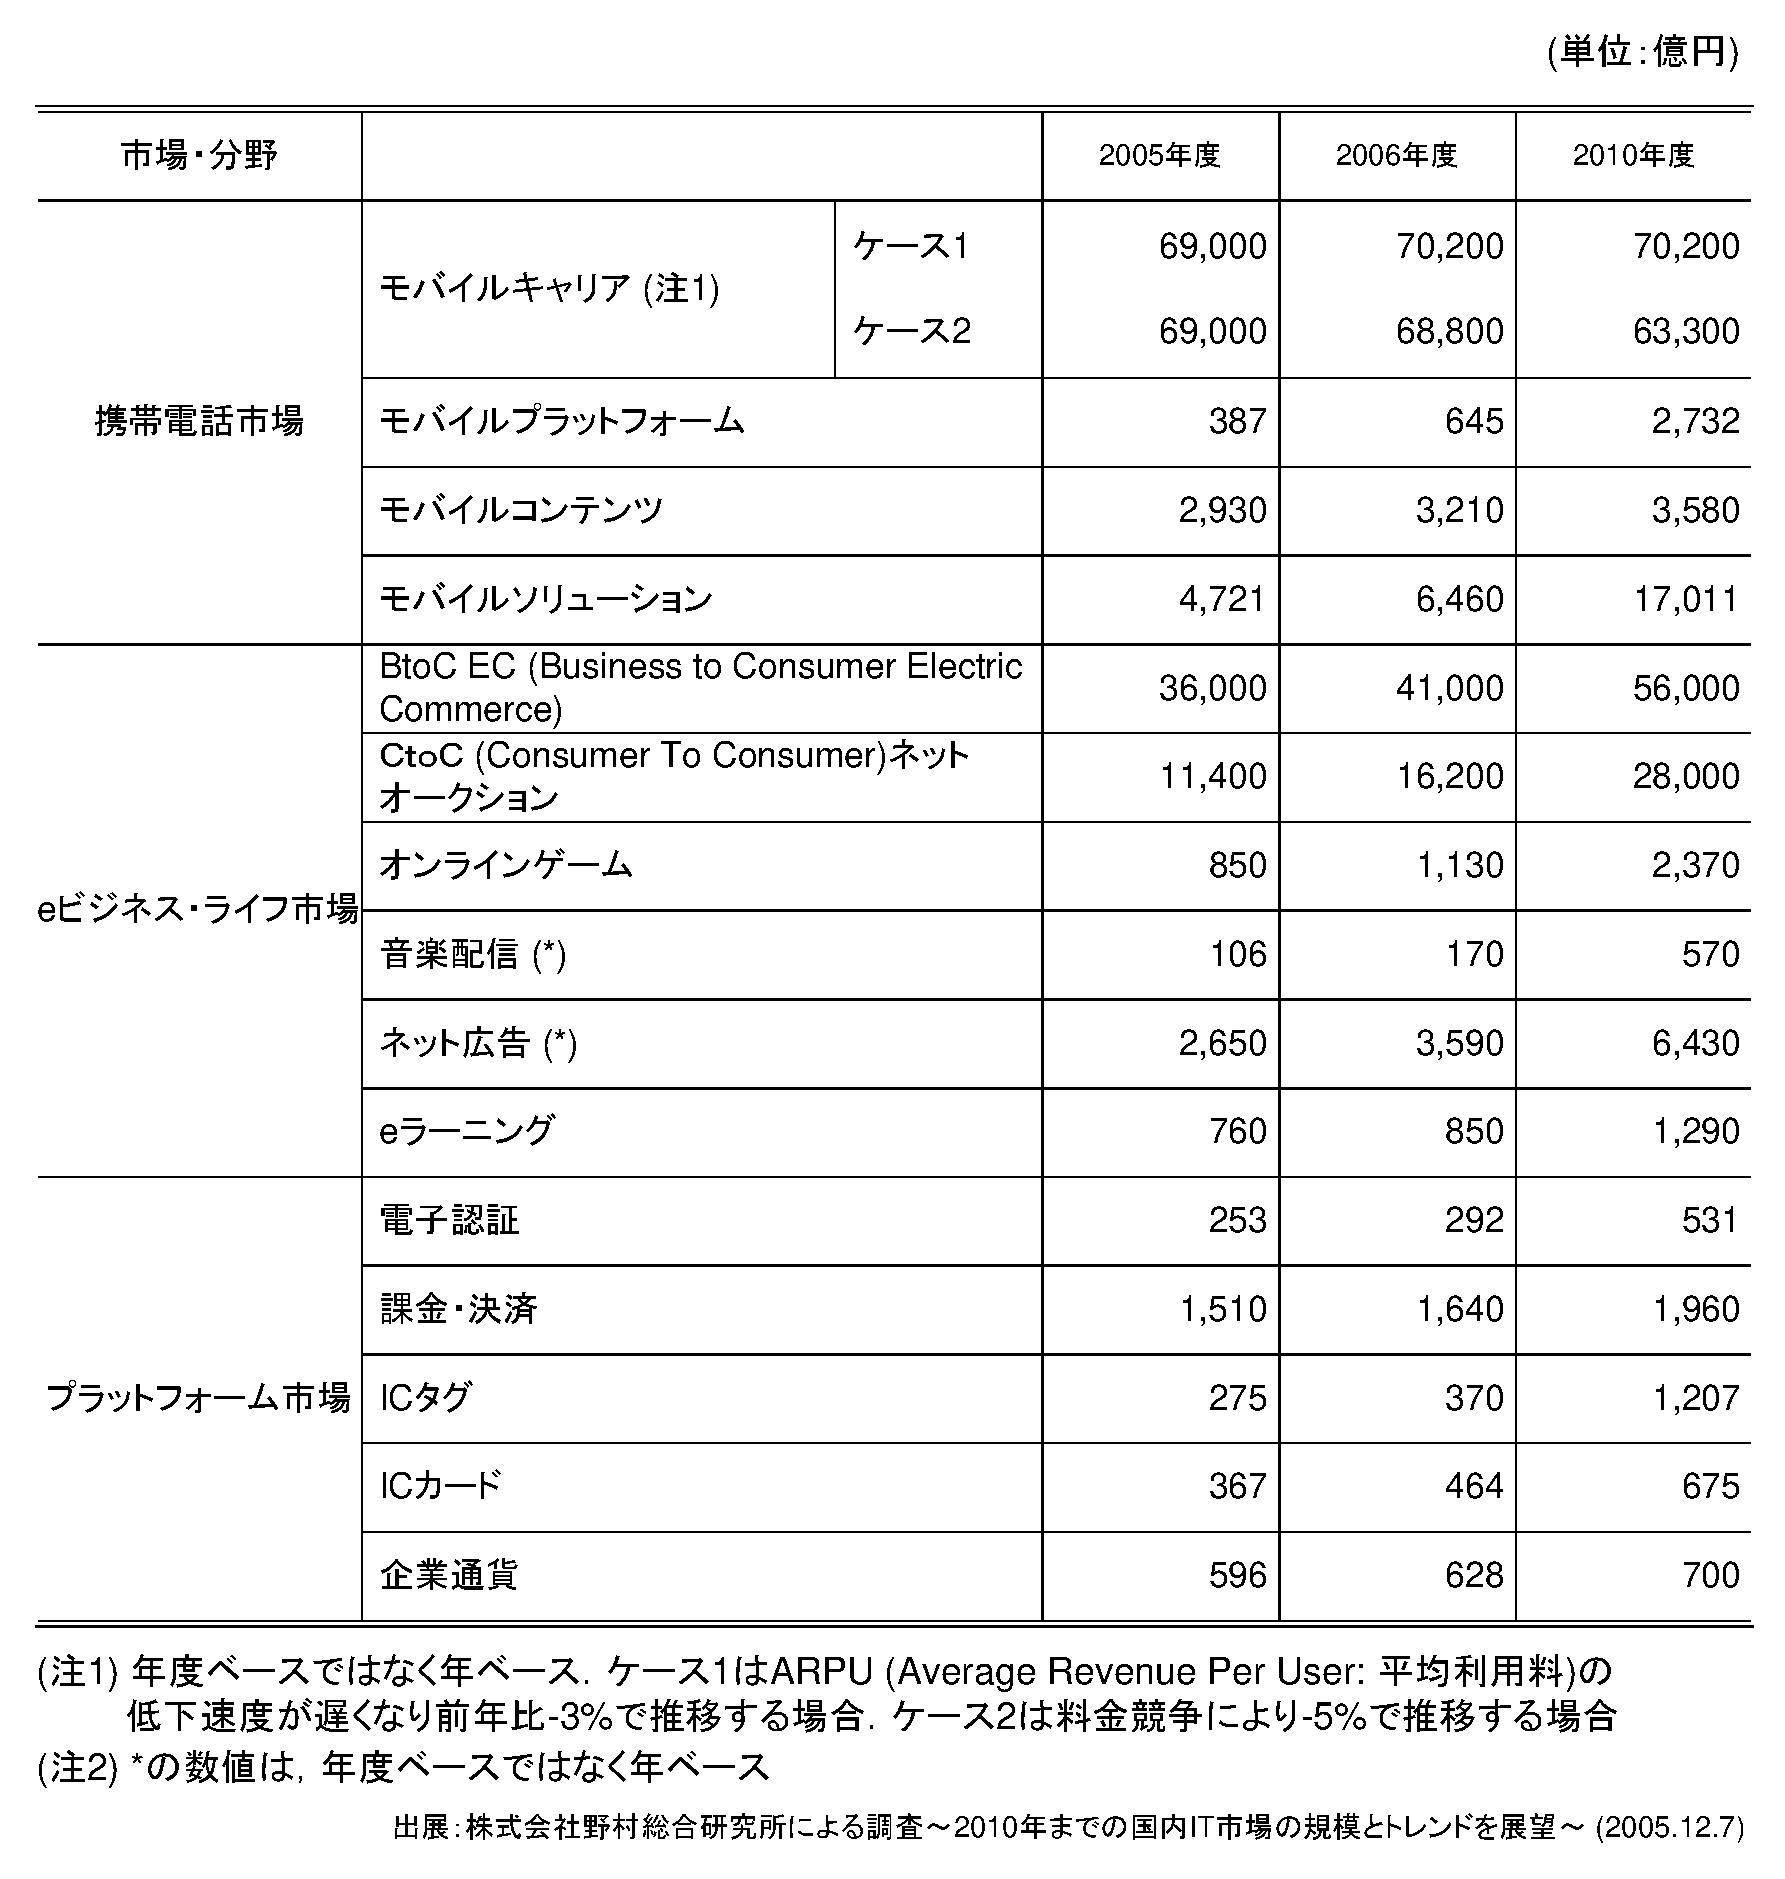
\includegraphics[width = 14cm,  height = 14cm,  keepaspectratio,  clip]{./pics/nomura_mobile.eps}
			\end{center}
		\label{nomura_mobile}
%		\vspace{-10mm}
	\end{table}%


以上の背景から,今後ユーザが高品質かつ大容量のマルチメディアデータを手軽に取り扱う機会がますます増加することは
容易に推測できる.
ここで述べるマルチメディアデータとは,``文字だけでなく音声やカラー映像を駆使したリッチ・コンテンツ情報"\cite{shiinfj}を意味し,
マルチメディアとは,``電話,ラジオ,テレビ及びコンピュータなど,様々な機器が取り扱うデータを互いにリンクさせ,
融合させたもの"\cite{kahadbt04}
と定義することができる.
以下にマルチメディアデータが使用される具体的な例を以下に挙げる.

\begin{itemize}
\item ビデオ
	
	Video CD,DVD player,デジタルカメラ等

\item オーディオ,音声

	MP3プレーヤ,音声入力,音声自動翻訳等

\item グラフィックス

	デジタルテレビ,家庭用ゲーム機,アミューズメントマシン,カーナビゲーションシステム等

\item 通信・認識

	ロボット,指紋認証等
\end{itemize}

これらのアプリケーションが単体,もしくはいくつか組み合わさることにより,これからの
マルチメディア機器は,オーディオ,画像,グラフィックス等大量のマルチメディアデータをリアルタイムに処理する
高い性能が必要となるのは容易に推測できる.
また,これに加えて高スループットの通信機能,安全性の高いセキュリティ機能,及び高度な認識機能も
実装されると考えられる.

図 \ref{mlt_spc}に,現在及び今後求められるマルチメディアデータ処理の要求性能を示す.
図中では,マルチメディアアプリケーションに必要とされる基本的な演算性能を,GOPS (Giga Operations Per Second)で示した.
MPEG-4や現行のテレビの解像度を処理するMPEG-2のMP@ML (Mail Profile at Main Level)の動画像処理では,1 GOPS程度の高い性能が要求され,
デジタルテレビの機能と解像度を処理するMPEG-2のMP@HL (Mail Profile at High Level)の処理では,10 GOPS以上の性能が要求されることになる.
最新の研究では,
国際固体素子回路会議ISSCC2005 (International Solid-State Circuits Conference 2005)にて,富士通の研究グループが
32 bitマルチメディアプロセッサコアであるFR550を4つマルチコア化し,MPEG-2のMP@HLを51 GOPSで処理可能にしたという結果が報告されている
\cite{hjfr5505}.
MPEGや,Dolby-AC3等のオーディオ伸長処理では,それほど高い性能は要求されないが.音声自動翻訳では
100 GOPS程度と非常に高い性能が要求される.
主にゲーム機等のアミューズメントアプリケーションで必要となる,3次元グラフィックス処理では100 Mpps (Mega polygons per second)
のスループットを達成するのに,100 GOPS以上の処理能力を必要とする.
現在家庭用ゲーム機の1つとして広く普及している,プレイステーション2に使用されているLSI,Emotion Engineでは
66 Mppsの性能で3次元グラフィックスを処理している\cite{satggsl01j}.
通信認識においては,顔認識や動画像認識で5~100 GOPSと幅広い性能が求められる.
カーナビゲーション等の用途に今年度開発された,ルネサステクノロジの最新マルチメディアプロセッシングのコアであるSH7785は,
600 MHzで,1 GOPSというスループットでマルチメディアデータを処理することが可能である\cite{jaresh7785}.
以上より,マルチメディアデータ処理LSIには,大量のデータを高速に処理する性能が,今後益々求められることが分かる.

% figure*
	\begin{figure*}[tbh]
	\centering
		\begin{center}
			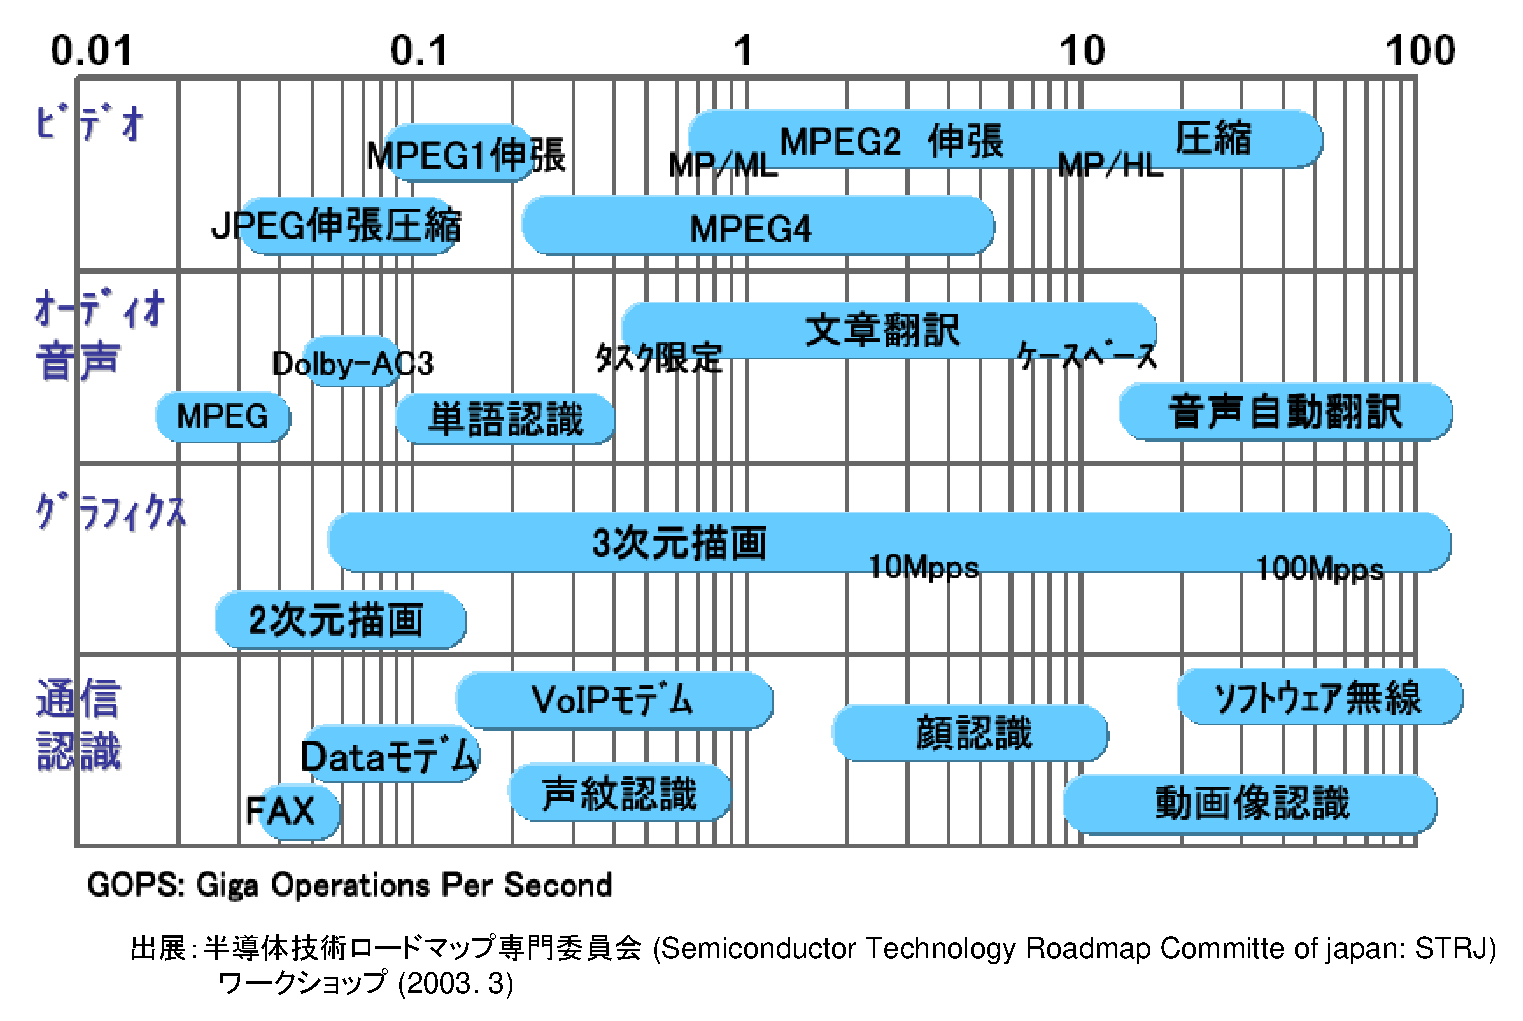
\includegraphics[width = 14cm,  height = 14cm,  keepaspectratio, clip]{./pics/mlt_spc.eps}
		\caption{マルチメディアデータ処理に要求される性能.}
		\label{mlt_spc}
		\end{center}
	\end{figure*}%	
%figure*

次に,マルチメディアデータを効率よく処理するためのアルゴリズムについて述べる.
一般に,マルチメディアアプリケーションに適用されるアルゴリズムは,音声や動画等の
アナログの情報を,処理速度に加え高精度かつ高圧縮に処理することが求められる.
マルチメディアデータの中でも,ビデオデータは特に膨大でありデータ圧縮を施さなければ
通信速度や処理速度の向上率を必要以上に高めなければならなくなる.
図 \ref{mlt_alg}に,ビデオ圧縮伸長アルゴリズムの例を示す.
横軸がビットレート,縦軸が解像度であり,各アルゴリズムの処理範囲を表している.
主なビデオ圧縮伸長技術としては,ITU-T (International Telecommunication Union)の勧告である
H.261やH.263,ISO (International Organization for Standardization)の定めた国際標準である
MPEG-1,MPEG-2,及びMPEG-4がある.
H.261とH.263は電話回線を用いたTV会議用に開発された.
特にH.263はエラー耐性や圧縮率向上を図ったオプションが多数用意されており,
移動体通信にも適用可能となっている.
MPEG-1やMPEG-2は,ビデオCDやDVD等の画像観賞用に用いられている.
MPEG-4に関しては,1999年にバージョン1が国際標準となった比較的新しい規格であり,
広範囲のアルゴリズムをカバーできる仕様となっている.
また図中には示していないが,近年では圧縮率を向上させたH.264が2003年5月に勧告として承認されている.
以上のように,大量のデータを取り扱うマルチメディアデータ処理には,
高圧縮を実現するアルゴリズムが不可欠であり,これらのアルゴリズムを効率的に
処理することがマルチメディアデータ処理LSIに求められるのである.


% figure*
	\begin{figure*}[tbh]
	\centering
		\begin{center}
			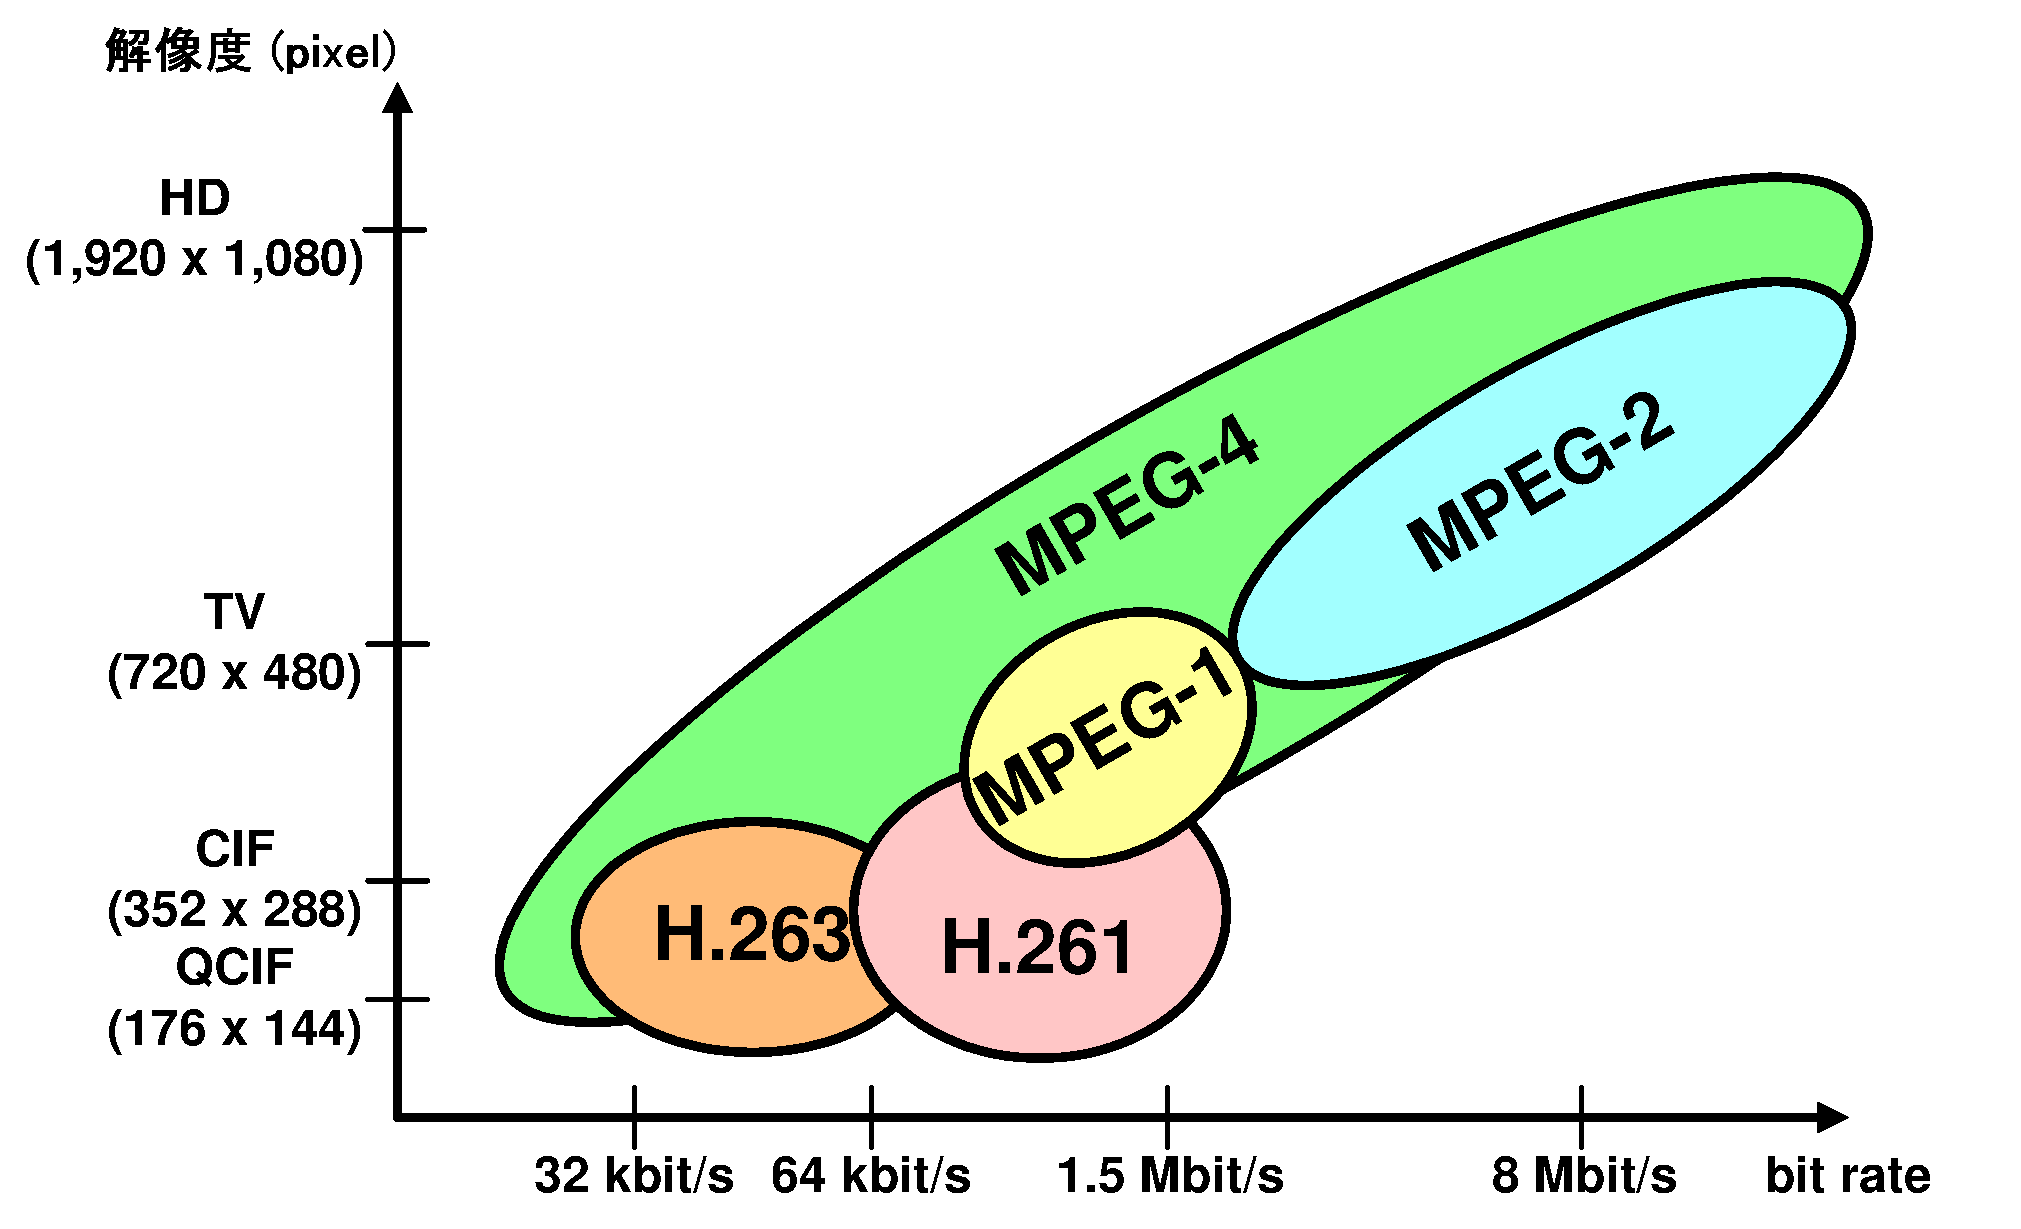
\includegraphics[width = 14cm,  height = 14cm,  keepaspectratio, clip]{./pics/mlt_alg.eps}
		\caption{ビデオ圧縮伸長技術.}
		\label{mlt_alg}
		\end{center}
	\end{figure*}%	
%figure*





\section{本研究の目的}
\label{lbl_cp1_mokuteki}

本研究では,\ref{lbl_cp1_gijyutu}節,及び\ref{lbl_cp1_rsrchpst}節の検討を通して,
プログラマブルであるという汎用的性質を持ちながら,
処理能力は専用ハードウェアに近いという設計思想の下に,
リアルタイムにマルチメディアデータを高速処理,高圧縮でき,
小面積かつ低消費電力であるマルチメディアデータ処理LSIアーキテクチャの開発を研究目的とする.

はじめに,マルチメディアデータ処理のボトルネックとなっているテーブルルックアップ処理に主眼を置く.
テーブルルックアップ処理の高速化には,機能メモリの一種であり,主として一致検索処理を高速に実現することのできる
CAMを利用する.
CAMは1956年に発表されたクライオトロン・カタログメモリ (Cryotron catalog memory)\cite{slacry}を起源とする,
高速に一致検索処理を行うことのできる機能メモリの一種であり,これまで様々な研究や実用化が行われてきた.
本論文では,CAMのアーキテクチャをベースとして,マルチメディアデータ処理LSIアーキテクチャの開発を行う.
また,モバイル機器をターゲットとした200 MHz前後の低い動作周波数で高速化を実現する手法として,
通常のCAMに複数の入出力ポートを付加した,
新しいアーキテクチャである,マルチポートCAMを適用する.
この適用によって,これまで実現が困難であった,テーブルルックアップ処理の並列化を検討する.
更に,上記のアーキテクチャにデータ圧縮を実現する機構を加え,
リアルタイム処理に加え高圧縮を実現するアーキテクチャを実現する.

次に,%CAMベースのテーブルルックアップ処理LSIアーキテクチャを検討した後に,
従来のプロセッシングアーキテクチャと比較して,大幅に並列度を向上させることで,
繰り返し演算処理を高速に実現できる,SRAMベースの超並列SIMD型プロセッシングアーキテクチャの開発を
行う.
そして,上記で述べたCAMベースのテーブルルックアップアーキテクチャと繰り返し演算処理SIMD型アーキテクチャを
融合させることで,マルチメディアデータをリアルタイム,プログラマブル,かつ高圧縮に処理することができる,
高性能CAMベースマルチメディアデータ処理LSIアーキテクチャの開発を行う.




